% THIS IS SIGPROC-SP.TEX - VERSION 3.1
% WORKS WITH V3.2SP OF ACM_PROC_ARTICLE-SP.CLS
% APRIL 2009
%
% It is an example file showing how to use the 'acm_proc_article-sp.cls' V3.2SP
% LaTeX2e document class file for Conference Proceedings submissions.
% ----------------------------------------------------------------------------------------------------------------
% This .tex file (and associated .cls V3.2SP) *DOES NOT* produce:
%       1) The Permission Statement
%       2) The Conference (location) Info information
%       3) The Copyright Line with ACM data
%       4) Page numbering
% ---------------------------------------------------------------------------------------------------------------
% It is an example which *does* use the .bib file (from which the .bbl file
% is produced).
% REMEMBER HOWEVER: After having produced the .bbl file,
% and prior to final submission,
% you need to 'insert'  your .bbl file into your source .tex file so as to provide
% ONE 'self-contained' source file.
%
% Questions regarding SIGS should be sent to
% Adrienne Griscti ---> griscti@acm.org
%
% Questions/suggestions regarding the guidelines, .tex and .cls files, etc. to
% Gerald Murray ---> murray@hq.acm.org
%
% For tracking purposes - this is V3.1SP - APRIL 2009

\documentclass{acm_proc_article-sp}

\begin{document}


\title{Sentiment Analysis using Keyboard and Mouse Dynamics for the
  Sequencing of Computer Programming Exercises}

%
% You need the command \numberofauthors to handle the 'placement
% and alignment' of the authors beneath the title.
%
% For aesthetic reasons, we recommend 'three authors at a time'
% i.e. three 'name/affiliation blocks' be placed beneath the title.
%
% NOTE: You are NOT restricted in how many 'rows' of
% "name/affiliations" may appear. We just ask that you restrict
% the number of 'columns' to three.
%
% Because of the available 'opening page real-estate'
% we ask you to refrain from putting more than six authors
% (two rows with three columns) beneath the article title.
% More than six makes the first-page appear very cluttered indeed.
%
% Use the \alignauthor commands to handle the names
% and affiliations for an 'aesthetic maximum' of six authors.
% Add names, affiliations, addresses for
% the seventh etc. author(s) as the argument for the
% \additionalauthors command.
% These 'additional authors' will be output/set for you
% without further effort on your part as the last section in
% the body of your article BEFORE References or any Appendices.

\numberofauthors{3} %  in this sample file, there are a *total*
% of EIGHT authors. SIX appear on the 'first-page' (for formatting
% reasons) and the remaining two appear in the \additionalauthors section.
%
\author{
% You can go ahead and credit any number of authors here,
% e.g. one 'row of three' or two rows (consisting of one row of three
% and a second row of one, two or three).
%
% The command \alignauthor (no curly braces needed) should
% precede each author name, affiliation/snail-mail address and
% e-mail address. Additionally, tag each line of
% affiliation/address with \affaddr, and tag the
% e-mail address with \email.
%
% 1st. author
\alignauthor
Amaury Hern\'andez-Aguila\\
       \affaddr{Tijuana Institute of Technology}\\
       \affaddr{Calzada Tecnologico s/n, Tomas Aquino}\\
       \affaddr{Tijuana, Mexico}\\
       \email{amherag@tectijuana.edu.mx}
% 2nd. author
\alignauthor
Mario Garc\'ia-Valdez\\
       \affaddr{Tijuana Institute of Technology}\\
       \affaddr{Calzada Tecnologico s/n, Tomas Aquino}\\
       \affaddr{Tijuana, Mexico}\\
       \email{mario@tectijuana.edu.mx}
% 3rd. author
\alignauthor
Alejandra Mancilla\\
       \affaddr{Tijuana Institute of Technology}\\
       \affaddr{Calzada Tecnologico s/n, Tomas Aquino}\\
       \affaddr{Tijuana, Mexico}\\
       \email{alejandra.mancilla@gmail.com}
\and  % use '\and' if you need 'another row' of author names
% 4th. author
\alignauthor
% 5th. author
\alignauthor
% 6th. author
\alignauthor
}
% There's nothing stopping you putting the seventh, eighth, etc.
% author on the opening page (as the 'third row') but we ask,
% for aesthetic reasons that you place these 'additional authors'
% in the \additional authors block, viz.

% Just remember to make sure that the TOTAL number of authors
% is the number that will appear on the first page PLUS the
% number that will appear in the \additionalauthors section.

\maketitle
\begin{abstract}
This work presents a method based on keystroke and mouse dynamics for
the analysis of a student's sentiments while interacting with an
intelligent tutoring system called Protoboard (http://protoboard.org/), which focuses on the
teaching of computer programming. The data gathered by the keystroke
and mouse dynamics could be used % could be used as a factor for recommending  
%Es importante que se entienda que estos datos se usan en conjunto con
%otros, por ejemplo el nivel de dificultad de los ejercicios.
as a factor for recommending a sequence of programming
exercises for a student that is interacting with the system.
This sequence of exercises is expected to affect the student's mental states during
the course of the programming lessons and exercises, with the purpose
of enhancing the learning experience of the student. 
% Como sabemos que la secuencia de ejercicios afectan el estado mental del estudiante? Siempre hay que ser cautelosos con las afirmaciones, que evidencia tenemos de esto? Estamos peleando en un terreno hostil, ya que los que hacen sistemas de recomendacion no entran mucho en la discusión de sentimientos. Es mejor aligerar las cosas con algo como: Is expected that this sequence of exercises will affect the student's mental states during...
%The method focuses on maximizing or minimizing /// Original 
%¿Que te parece decir mejor algo como: The recommender algorithm considers a (measure?) of six mental states..? Es más fácil de comprobar, digamos estás aburrido puedo considerar eso para recomendarte un ejercicio. No siempre será posible y no sabemos que sentimientos serían los que debemos considerar etc. Lo mejor es partir de la idea de que cientificamente no sabemos muchas cosas.
% No necesariamente vamos minimizar o maximizar los estados, ¿se habla de esto en los otros papers que haz leido?
%Leyendo otra vez creo que esta mejor hablar del método de los
%keystrokes

The recommender algorithm considers a measure of six mental states:
frustration, boredom, relaxation, distraction, concentration, and excitement.

%The method focuses on predicting a degree of % No se si es degree //Editado lo malo es que si lo aceptas hay que modificar un poco lo de abajo para que tenga sentido, ya que se repite lo de prediction  
%six mental states: frustration,
%boredom, relaxation, distraction, concentration, and excitement. 
For the prediction of these mental states, an artificial neural
network classifies a student according to their keyboard and mouse dynamics into different degrees of the mental states. 
%En este caso estas mezclando dos cosas distintas: la clasificación asigna una clase a cada objeto (a menos que sea difusa) y la predicción si puede asignar el nivel esperado de cada métrica. Creo que solo estas prediciendo. 
These degrees are used 
for a recommender % as variables in a recommender system algorithm wich assignes a recommendation measure to each exercise. The algorithm also considers: the student's performance in previous excersises and the exercise level of difficulty, 
system to determine a better sequencing of the exercises to be
presented to the student. A prototype of the system has been
developed, and is currently being tested.
%  

\end{abstract}
%172 words

\category{H.5.2}{User Interfaces}{Input devices and strategies}

\terms{Human Factors} % NOT required for Proceedings

\keywords{Affective Computing, Intelligent Tutoring Systems, Keyboard
  Dynamics, Mouse Dynamics, Emotion Sensing, Neural Networks}

\section{Introduction}

\subsection{Intelligent Tutoring Systems}
\label{ITSs}

The prototype that is being developed falls under the category of
Intelligent Tutoring Systems (ITS). An ITS is any software which
objective is to facilitate a student's learning through the use of
different tools, such as natural language processing, semantic web or
machine learning. In this case, Protoboard uses machine learning
techniques to predict a student's mental states and emotions, and use
these emotions as input to a recommender system. This is achieved
using neural networks as the classification model, and keystroke and
mouse dynamics as the input to this model.

The recommendation is performed over an implementation of the IMS Simple
Sequencing (SS) specification. SS allows us to establish a precondition
rule on each of the learning objects in a learning
activity. Precondition rules are defined to restrain a learning object
from being shown to the user, and allow other objects to be shown.

%145 words

\subsection{Affective Computing}
One of the areas of study that Protoboard is leveraging is Affective
Computing, a branch of computer science which studies how to interpret
and emulate human emotions. The platform recognises how a student was
feeling during their interaction with a learning object, such as a
video, a programming exercise or a quiz, and these predictions can
then be used to recommend what the next learning object will be, in
order to maximise or minimise an emotion.

The resulting predicted values of a user's mental states and emotions
can be used for other content adaptation tasks in the system, e.g.,
estimating if a student needs more exercises of certain learning style
(visual, verbal, aural, etc.), or as input to other processes, as in
the case of a module for predicting if a student needs more hints, or
a module that determines if a student is cheating in a test.

%149 words

\subsection{IMS Simple Sequencing}

"IMS Simple Sequencing (IMS SS) is a specification used to describe
paths through a collection of learning activities. IMS SS declares
the relative order in which electronic learning activities are to be
presented to a learner and the conditions under which a resource is
selected, delivered, or skipped during
presentation. \cite{bailey2007ims}"

As mentioned in \ref{ITSs}, precondition rules are given to the
learning objects in the learning activities in Protoboard, which allow
us to control the sequence in which these objects are presented to the
user. The neural network models in Protoboard send predicted values
for a student's mental states to the implementation of IMS SS after the
completion of an exercise, and then Simple Sequencing decides what
activity to show next.

%123 words

\subsection{Recommender System}

\subsection{Artificial Neural Networks}
\label{ANN}
%0 words

\subsection{Keystroke Dynamics}
\label{KD}

Keystroke Dynamics (KD) is the information about the rhytm and manner
in which an individual presses the keys of a keyboard or
keypad. Usually, there are two events that can be recorded from the
interaction with a keyboard: a keydown event, which occurs when a key
is fully pressed and hasn't been released; and a keyup event, which
occurs when a key has been released of its pressed state. These events
are recorded alongside the time when they occured.

The information recorded often needs to be preprocessed in order to
serve as input to other processes, such as identificaiotn and
authentication procedures, and emotion interpretation in software
systems. In general, this preprocessing usually results in a
collection of lapses of time between one event and another in the
keypresses.

%129 words

\subsection{Mouse Dynamics}

Mouse Dynamics (MD) is an extraction and processing of information
very similar to KM \ref{KD}, but with some key differences. The first
notable difference is that a mouse usually has only from three to four
keys (left button, right button, mouse wheel button, and some mouse
models have a middle button) that a user can press. But some mouse
models present seven buttons or more, mainly those designed for video
games. This can pose a problem, because computer mouses lack the
standardization that computer keyboards present. The second difference 
is that a computer mouse can be tracked by its position in a plane.

Similar to KD, MD usually record the keydown and keyup events of its
different buttons, and additionally, different mouse positions can be
tracked, usually with a time interval between each record.

%135

\subsection{Experience Sampling Method}
\label{ESM}

Experience Sampling Method (ESM) is a research methodology in which a
group of questions is asked to a participant of an experiment about
their feelings, opinions, ideas or emotions, at certain intervals of
time. The method is mainly designed to gather subjective data from
human beings.

ESM is used in this work to ask the users of Protoboard, every time
they finish an excersie, how they were feeling during their solving of
the programming problem.

%75 words

\subsection{Protoboard}

\subsection{Flow}

Flow is a mental state where an individual, while performing an
activity, experiences a feeling of focus or deep mental
involvement, and enjoys the course of the activity \cite{cit:4}. Flow
is closely related to motivation, the main difference being that
motivation is the purpose or psychological cause of any action
\cite{cit:16}. Thus, a person can be very motivated to execute and
continue the execution of certain action, but not necessarily be in a
state of flow.

%80 words

\section{Proposed Method}

This work focuses on implementing a module for Protoboard (http://app.protoboard.org/) that
records, among other data, keystroke and mouse dynamics, which then
will be preprocessed for a neural network to decide if a user was
experiencing certain emotional states. The resulting predicted values
will then be used for a recommender system for deciding what is the
appropriate sequence of learning objects that should maximise and
minimise specific emotions in the student. The predicted emotion
values will be used for other processes and tasks in the system, such
as the recommendation of learning objects of a specific learning
style, and classifying a student as being cheating during the course
of a learning activity or not.

%112 words

\subsection{Keystroke and Mouse Dynamics}

For the recording of the keypresses of the keyboard and mouse from a
student, a JavaScript script was created. This script is attached to
every programming exercise in a learning activity, as these are the
learning objects where a user would write the most. Every keydown and
keyup event is recorded, as well as the time in milliseconds in which the event
occurred. All of these events are temporarily stored in the web
browser, and when the user chooses to continue to the next activity,
these records are sent to the server, where they get stored.

Mouse positions are recorded every 100 milliseconds, only if the
system detects that a change of position occurred. If no movement has
occurred since the last reading, a record isn't stored.

%127 words

\subsection{Experience Sampling Method}
\label{PM-ESM}

After every programming excersice in a learning activity in
Protoboard, an ESM \ref{ESM} is applied to the student to measure their levels
of boredom, relaxation, distraction, concentration, and
excitement. The students are instructed to answer the ESM,
according to how they were feeling during their experience with the
programming exercise they just solved, or tried to solve. The
questions, or statements, presented to the student are the following:

\begin{itemize}
  \item I was feeling frustrated
  \item I was feeling bored
  \item I was feeling relaxed
  \item I was feeling distracted
  \item I was feeling concentrated
  \item I was feeling excited
\end{itemize}

and a series of five likert-style possible answers are shown below the
statements: "I strongly agree", "I agree", "Neutral", "I disagree",
and "I strongly disagree." Figure \ref{fig:ESM-test} shows a sample
ESM test (in Spanish) as presented in Protoboard.

\begin{figure}
  \centering
  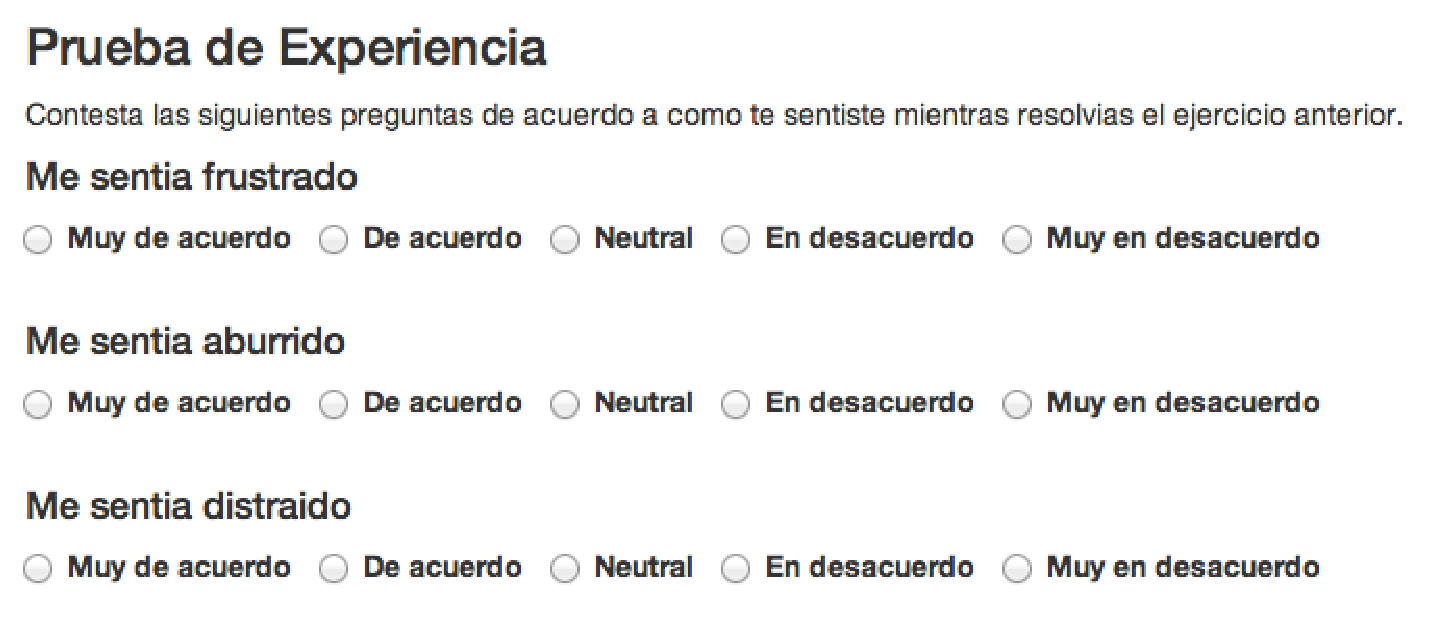
\epsfig{file=esm-test.eps, width=3.5in}
  \caption{A sample of three of the six statements a student must
    respond to in the Experience Sampling Method test.}
  \label{fig:ESM-test}
\end{figure}

If users try to skip answering one of the questions, the system
will forbid them to continue. If the user answers all the questions
and continues to the next activity, the answers will be recorded in a
database in the server.

%195 words

\subsection{Neural Network}

An artificial neural network (see \ref{ANN}) is trained using the data generated
by the users while solving the programming exercises in the learning
activity, and tries to match, as outputs, the data generated by the
answers in the ESM tests that followed each programming exercise.

As Protoboard is currently under development, a definite architecture
for the artificial neural networks doesn't exist yet, although we are
expecting that a very basic architecture could be sufficient.

%75 words

\subsection{Emotions}

As has been noted before, in this work we are measuring six different
emotions from the user: frustration, boredom, relaxation, distraction,
concentration, and excitement. These emotions were chosen as they are
expected to have a correlation with the mental state of flow \ref{flow}.

%44 words

\bibliographystyle{abbrv}
\bibliography{sigproc}  % sigproc.bib is the name of the Bibliography in this case

\balancecolumns
% That's all folks!
\end{document}
